\documentclass[a4paper,12pt]{article}
\usepackage[top=2cm, bottom=2cm, left=2cm, right=2.5cm]{geometry}
\usepackage[utf8]{inputenc}
\usepackage[brazil]{babel}
\usepackage{amsmath, amsfonts, amssymb}
\usepackage{pifont} % Usado para especificar os simbolos em \begin{itemize} \item
\usepackage{hyperref} % Usado para adicionar hiperlinks com o comando p.ex: \href{http://www.latex-tutorial.com}{LaTeX-Tutorial}.
\usepackage{times} % Para usar a fonte Times New Roman no documento inteiro
\usepackage{graphicx} % Para incluir no documento figuras
\usepackage{float}

\begin{document}

\title{{\huge Capítulo 21 - Análise Combinatória - Métodos de Contagem} \\ 
  \, \linebreak \linebreak \linebreak Exercícios Respondidos, Básicos, Complementares e Questões de Vestibular
}
\date{}

\maketitle 

\begin{figure}[htb]
 \centering
 
\includegraphics[scale=0.4]{../../imagens/FOTO-PERFIL-DANIEL-CLAUDINO-2020.png}
\end{figure}

\begin{center}
  \begin{large}
    {\huge Daniel de Lima Claudino \linebreak \linebreak} 
  \end{large}
\end{center}

\begin{flushright}
  \begin{small}
    {\large \textbf{Referência Bibliográfica}\\PAIVA, Manoel Rodrigues. \textbf{Matemática}. Vol. 2. São Paulo: Moderna, 2004.} 
  \end{small}
\end{flushright}

\vfill

\begin{center}
  \begin{large}
    12 de Dezembro de 2022
  \end{large}
  
\end{center}

\thispagestyle{empty} % Não numera esta página

\newpage
\setcounter{page}{0}

\tableofcontents

\listoffigures

\listoftables

\thispagestyle{empty}% Não numera esta página

\newpage

\section{Mapa Mental - Análise Combinatória}

\setcounter{figure}{0}
\begin{figure}[htb]
\centering
\caption{Mapa Mental - Análise Combinatória}
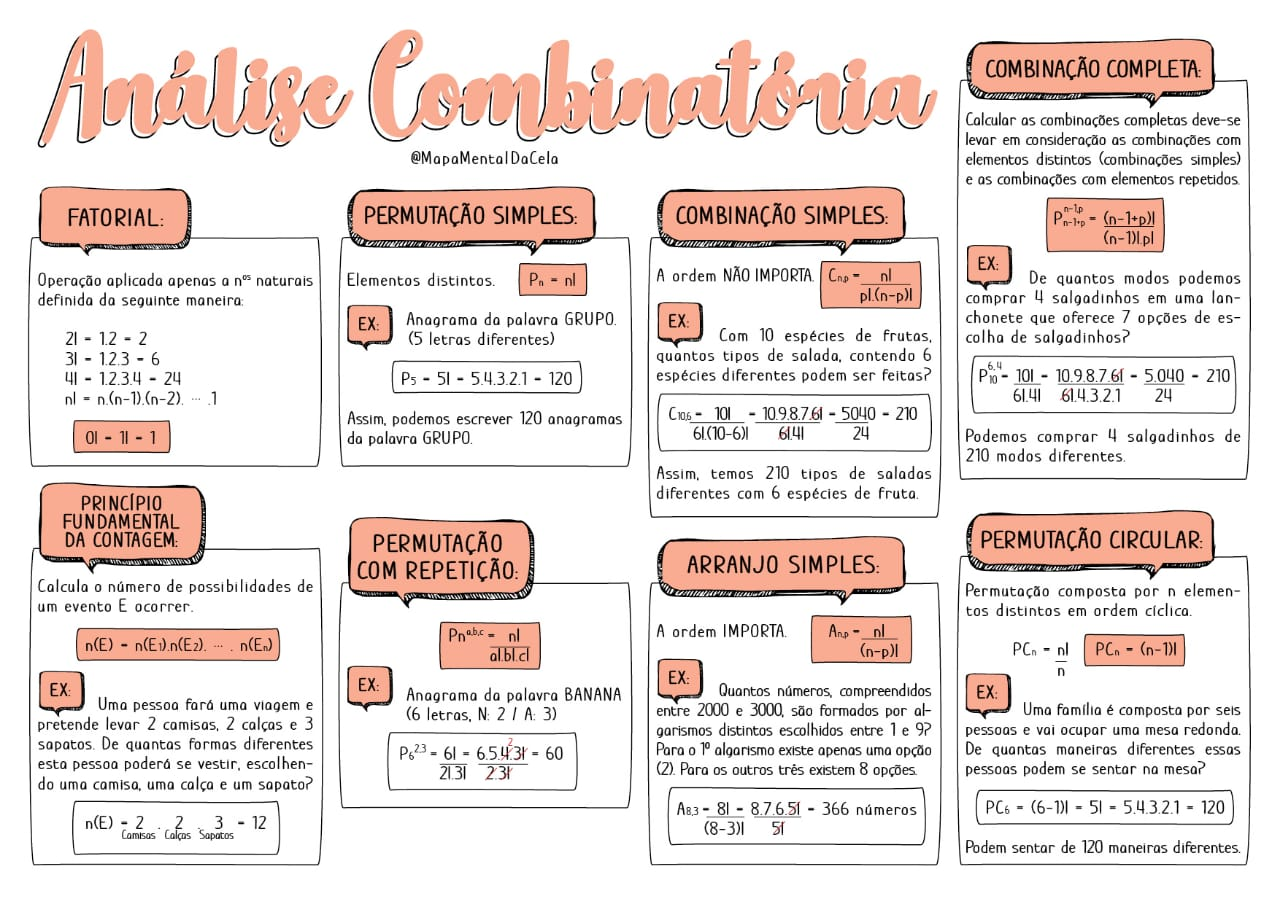
\includegraphics[scale=0.35]{../../imagens/mapa-mental-analise-combinatoria.jpeg}
\label{mapa-mental-analise-combinatoria}
Fonte:\href{https://infinittusexatas.com.br/analise-combinatoria-resumos-e-mapas-mentais/}{Site Infinittus - Conhecimento nas medidas exatas}
\end{figure}

\section{Exercícios Resolvidos}

\begin{enumerate}

\item[\textbf{R1}] Uma montadora de automóveis apresenta um carro em \textbf{quatro modelos} diferentes e em \textbf{cinco cores} diferentes. Um consumidor que quiser arquirir esse veículo terá quantas opções de escolha ?

  \begin{itemize}
    \item[\ding{172}] \textbf{O que contar?:} Quantas opções de escolha de veículo o consumidor terá ?
    \item[\ding{173}] \textbf{Restrições do(s) Experimento(s):} Nenhuma.
    \item[\ding{174}] \textbf{Experimento 1:} Escolher uma das opções de modelo. $n_{1}$ possui 5 resultados possíveis.
    \item[\ding{175}] \textbf{Experimento 2:} Escolher uma das opções de cor. $n_{2}$ possui 4 resultados possíveis.
    \item[\ding{176}] \textbf{Cálculo:} Pelo princípio fundamental da contagem (PFC), o experimento composto 1 e 2, nessa ordem, tem $n_{1} \times n_{2}$ resultados possíveis, ou seja, $5 \times 4 = 20$ opções de escolha.
    \item[\ding{177}] \textbf{Conclusão:}  existem 20 opções de escolha de veículos para o consumidor.
  \end{itemize}
  
  \newpage

\item[\textbf{R2}] Quantos números naturais de três algarismos podem ser formados com os algarismos $A = \{1, 2, 6, 8, 9\}$ ?
   \begin{itemize}
    \item[\ding{172}] \textbf{O que contar?:} Quantos números naturais de três algarismos podem ser formados com os algarismos dados.
    \item[\ding{173}] \textbf{Restrições do(s) Experimento(s):} Nenhuma.
    \item[\ding{174}] \textbf{Experimento 1:} $E_1$ = Preencher a posição das unidades com um dos algarismos dados.\\ Sendo $n_{1}$ o número de resultados possíveis do \textbf{experimento 1}, $n_{1}$ possui $n(A)$ resultados possíveis, ou seja, $n_{1} = n(A) = 5$.
    
    \item[\ding{175}] \textbf{Experimento 2:} $E_2$ = Preencher a posição das dezenas com um dos algarismos dados.\\ Sendo $n_{2}$ o número de resultados possíveis do \textbf{experimento 2}, $n_{2}$ possui $n(A)$ resultados possíveis, já que nenhuma restrição existe para realizarmos o experimento, ou seja, $n_{2} = n(A) = 5$.
    
    \item[\ding{176}] \textbf{Experimento 2:} $E_3$ = Preencher a posição das centenas com um dos algarismos dados.\\ Sendo $n_{1}$ o número de resultados possíveis do \textbf{experimento 2}, $n_{3}$ possui $n(A)$ resultados possíveis, já que nenhuma restrição existe para realizarmos o experimento, ou seja, $n_{3} = n(A) = 5$.
    
    \item[\ding{177}] \textbf{Cálculo:} Pelo princípio fundamental da contagem (PFC), os experimentos 1, 2 e 3 apresentam, respectivamente, $n_{1},\, n_{2} \textrm{ e } n_{3}$ resultados possíveis, logo o experimento composto 1, 2 e 3 possuem, nessa ordem, $n_{1} \times n_{2} \times n_{3}$ ou $5 \times 5 \times 5 = 125$ resultados possíveis.
    \item[\ding{178}] \textbf{Conclusão:} Podemos formar \textbf{125 números naturais de três algarismos} com os números dados.
  \end{itemize}
  
\item[\textbf{R3}] Quantos números naturais de três algarismos \textbf{distintos} podem ser formados com os algarismos $A = \{1, 2, 6, 8, 9\}$ ?
   \begin{itemize}
    \item[\ding{172}] \textbf{O que contar?:} Quantos números naturais de três algarismos \textbf{distintos} podem ser formados com os algarismos dados.
    \item[\ding{173}] \textbf{Restrições do(s) Experimento(s):} Os números escolhidos em cada experimento devem ser distintos.
    \item[\ding{174}] \textbf{Experimento 1:} $E_1$ = Preencher a posição das unidades com um dos algarismos dados.\\ Sendo $n_{1}$ o número de resultados possíveis do \textbf{experimento 1}, $n_{1}$ possui $n(A)$ resultados possíveis, ou seja, $n_{1} = n(A) = 5$.
    \item[\ding{175}] \textbf{Experimento 2:} $E_2$ = Preencher a posição das dezenas com um dos algarismos dados.\\ Sendo $n_{2}$ o número de resultados possíveis do \textbf{experimento 2}, $n_{2}$ possui $n(A)-1$ resultados possíveis,pois um dos algarismos já foi escolhido no experimento 1, ou seja, $n_{2} = n(A)-1 = 5 - 1 = 4$.
    \item[\ding{176}] \textbf{Experimento 3:} $E_3$ = Preencher a posição das centenas com um dos algarismos dados.\\ Sendo $n_{3}$ o número de resultados possíveis do \textbf{experimento 3}, $n_{3}$ possui $n(A)-2$ resultados possíveis,pois um dos algarismos já foi escolhido no \textbf{experimento 1} e outro no \textbf{experimento 2}, ou seja, $n_{2} = n(A) - 2 = 5 - 2 = 3$.   
    \item[\ding{177}] \textbf{Cálculo:} Pelo princípio fundamental da contagem (PFC), os experimentos 1, 2 e 3 apresentam, respectivamente, $n_{1},\, n_{2} \textrm{ e } n_{3}$ resultados possíveis, logo o experimento composto 1, 2 e 3 possuem, nessa ordem, $n_{1} \times n_{2} \times n_{3}$ ou $5 \times 4 \times 3 = 60$ resultados possíveis.
    \item[\ding{178}] \textbf{Conclusão:} Podemos formar \textbf{60 números naturais de três algarismos distintos} com os números dados.
  \end{itemize}
  
\item[\textbf{R4}] Quantos números naturais de três algarismos \textbf{distintos} podem ser formados com os algarismos $A = \{0, 1, 2, 6, 8\}$ ?
   \begin{itemize}
    \item[\ding{172}] \textbf{O que contar?:} Quantos números naturais de três algarismos \textbf{distintos} podem ser formados com os algarismos dados.
    
    \item[\ding{173}] \textbf{Restrições do(s) Experimento(s):}
      \begin{enumerate}
    		\item[a)] Os números escolhidos em cada experimento devem ser distintos.
    		\item[b)] A posição da \textbf{centena} não pode conter o número zero ( 0 ), pois, nesse caso, o número natural formado não terá três algarismos, e sim dois.
      \end{enumerate}
    \item[\ding{174}] \textbf{Experimento 1:} $E_1$ = Preencher a posição das centenas com um dos algarismos dados, observando as duas restrições apontadas do experimento.\\ Lembrando que o zero não pode ser excolhido. Sendo $n_{1}$ o número de resultados possíveis do \textbf{experimento 1}, $n_{1}$ possui $n(A)$ resultados possíveis, ou seja, $n_{1} = n(A)-1 = 4$.
    
    \item[\ding{175}] \textbf{Experimento 2:} $E_2$ = Preencher a posição das dezenas com um dos algarismos dados, observando as duas restrições apontadas do experimento.\\ Lembrando que: (1) Já foi escolhido o algarismo das centenas e (2) para casa das dezenas o zero pode ser escolhido.\\ Sendo $n_{2}$ o número de resultados possíveis do \textbf{experimento 2}, $n_{2}$ possui $n(A)-1$ resultados possíveis,pois um dos algarismos já foi escolhido no experimento 1 e o zero pode ser escolhido, ou seja, $n_{2} = n(A)-1 = 5 - 1 = 4$.
    
    \item[\ding{176}] \textbf{Experimento 3:} $E_2$ = Preencher a posição das unidades com um dos algarismos dados, observando as duas restrições apontadas do experimento.\\ Lembrando que: (1) Já foi escolhido o algarismo das centenas e das dezenas e (2) para casa das unidades o zero pode ser escolhido.\\ Sendo $n_{2}$ o número de resultados possíveis do \textbf{experimento 2}, $n_{2}$ possui $n(A)-2$ resultados possíveis,pois um dos algarismos já foi escolhido no experimento 1, outro algarismo no experimento 2 e o zero pode ser escolhido, ou seja, $n_{2} = n(A)-2 = 5 - 2 = 3$.
      
    \item[\ding{177}] \textbf{Cálculo:} Pelo princípio fundamental da contagem (PFC), os experimentos 1, 2 e 3 apresentam, respectivamente, $n_{1},\, n_{2} \textrm{ e } n_{3}$ resultados possíveis, logo o experimento composto 1, 2 e 3 possuem, nessa ordem, $n_{1} \times n_{2} \times n_{3}$ ou $4 \times 4 \times 3 = 48$ resultados possíveis.
    
    \item[\ding{178}] \textbf{Conclusão:} Podemos formar \textbf{48 números naturais de três algarismos distintos} com os números dados.
  \end{itemize}
  
\item[\textbf{R5}] Quantos divisores naturais possui o número 72?
   \begin{itemize}
    \item[\ding{172}] \textbf{O que contar?} Quantos divisores naturais possui o número 72.
    
    \item[\ding{173}] \textbf{Restrições do(s) Experimento(s):} Nenhum.

    \item[\ding{174}] Fatoramos o número 72.
    
      \begin{table}[H]
        \centering
        Fatoração do número 72 \\
        \begin{tabular}{c|c}
     	  72 & 2 \\
	      36 & 2 \\
          18 & 2 \\
          9 & 3 \\          
          3 & 3 \\ \hline
          1 & $2^4 \cdot 3^2$ \\     
       \end{tabular}
       \label{fatoracao-numero-72}       
     \end{table}

    
    \item[\ding{175}] A partir da fatoração realizada no item 3, podemos construir uma lista de divisores do número 72. Qualquer número que pode ser escrito através do produto $2^{\{0..3\}} \times 3^{\{0..2\}} $, com $x \in \{0,1,2,3\}$ e $y \in \{0,1,2\}$, é um divisor de 72. Ou seja, os divisores são: 

      \begin{center}
     	$D(72)=\{2^0 \times 3^0,
     	2^0 \times 3^0,
     	2^0 \times 3^1,
     	2^0 \times 3^2,
     	2^1 \times 3^0,
     	2^1 \times 3^1,
     	2^1 \times 3^2,
     	2^2 \times 3^0,
     	2^2 \times 3^1,
     	2^2 \times 3^2,
     	2^3 \times 3^0,
     	2^3 \times 3^1,
     	2^3 \times 3^2
     	\}$ \\
     	ou \\
     	$D(72)=\{
        1,2,3,4,6,
        8,9,12,18,24,
        36,72\}
     	$
     \end{center}
        
    Um outra forma, mais genérica e rápida, de constatar que 72 possui 12 divisores é descobrir de quantas maneiras, no produto $2^{\{0..3\}} \times 3^{\{0..2\}} $, com $x \in \{0,1,2,3\}$ e $y \in \{0,1,2\}$, eu posso preencher o expoente do 2 e o expoente do 3. \\Percebe-se que, tal qual respondemos nas questões anteriores, pelo princípio fundamental da contagem (PFC), temos dois experimentos: $E_1 =$ Preencher o expoente do 2 e $E_2 =$ Preencher o expoente do 3. Sendo $n_{1}$ o número de resultados possíveis do experimento $E_1$ e $n_{2}$ o número de resultados possíveis do experimento $E_2$, temos que pelo PFC, o experimento composto $E_1$ e $E_2$, nessa ordem, apresenta $n_{1} \times n_{2}$ resultados possíveis, ou seja $4 \times 3 = 12$ números (divisores).
       
    \item[\ding{178}] \textbf{Conclusão:} O número 72 possui 12 divisores naturais
  \end{itemize}

\end{enumerate}



%
% --------------------   ESTRUTURA PADRÃO DE UMA QUESTÃO  ------------------------
% Observação: 
%    1) O "\item" abaixo precisa estar dentro de um \begin{itemize} ... \end{itemize}
%    2) Use CTRL + T para COMENTAR e CTRL + U para DESCOMENTAR
%    3) A resolução de uma questão é dividida da seguinte forma:
%      a) Enunciado da Questão
%      b) Apresentação de alguma figura (ilustração, esquema, mapamental) para auxiliar a resolução
%      c) Passos de 1 a 10 para resolver a questão
%
%\item[\textbf{QXX}] Coloque aqui o enunciado da questão ... ?
%   \begin{itemize}
%    \item[\ding{172}] \textbf{O que contar?:} .
%    
%    \item[\ding{173}] \textbf{Restrições do(s) Experimento(s):} .
%    
%    \item[\ding{174}] \textbf{Experimento 1:} $E_1$ = Preencher a posição das unidades com um dos algarismos dados.\\ Sendo $n_{1}$ o número de resultados possíveis do \textbf{experimento 1}, $n_{1}$ possui $n(A)$ resultados possíveis, ou seja, $n_{1} = n(A) = 5$.
%    
%    \item[\ding{175}] \textbf{Experimento 2:} $E_2$ = Preencher a posição das dezenas com um dos algarismos dados.\\ Sendo $n_{2}$ o número de resultados possíveis do \textbf{experimento 2}, $n_{2}$ possui $n(A)-1$ resultados possíveis,pois um dos algarismos já foi escolhido no experimento 1, ou seja, $n_{2} = n(A)-1 = 5 - 1 = 4$.
%    
%    \item[\ding{176}] \textbf{Experimento 3:} $E_3$ = Preencher a posição das centenas com um dos algarismos dados.\\ Sendo $n_{3}$ o número de resultados possíveis do \textbf{experimento 3}, $n_{3}$ possui $n(A)-2$ resultados possíveis,pois um dos algarismos já foi escolhido no \textbf{experimento 1} e outro no \textbf{experimento 2}, ou seja, $n_{2} = n(A) - 2 = 5 - 2 = 3$.   
%    
%    \item[\ding{177}] \textbf{Cálculo:} Pelo princípio fundamental da contagem (PFC), os experimentos 1, 2 e 3 apresentam, respectivamente, $n_{1},\, n_{2} \textrm{ e } n_{3}$ resultados possíveis, logo o experimento composto 1, 2 e 3 possuem, nessa ordem, $n_{1} \times n_{2} \times n_{3}$ ou $5 \times 4 \times 3 = 60$ resultados possíveis.
%    
%    \item[\ding{178}] \textbf{Conclusão:} Podemos formar \textbf{60 números naturais de três algarismos distintos} com os números dados.
%    
%  \end{itemize}


\end{document}